\section{Systems with known instability problems}

In order to stabilize the rocket in flight, a controller must be designed to stabilize the vertical position during flight. Experimenting such a system during flight is expensive and presents hazards.
Is there a system that has similar instability properties of rockets, and presents fewer contraries to experiment?

An Inverted Pendulum objective is to stabilize a stick which’s center of mass is above pivot point. The process is done using a horizontal force, resulting in a first degree of freedom rotation. This is similar to a rocket system. An example of an inverted pendulum would be humans. Adjustments are needed to maintain balance when standing, walking, or running. Flight are not required, therefore it is less restrictive to use and analyze an inverted pendulum.

\begin{figure}[htbp]
	\centering
	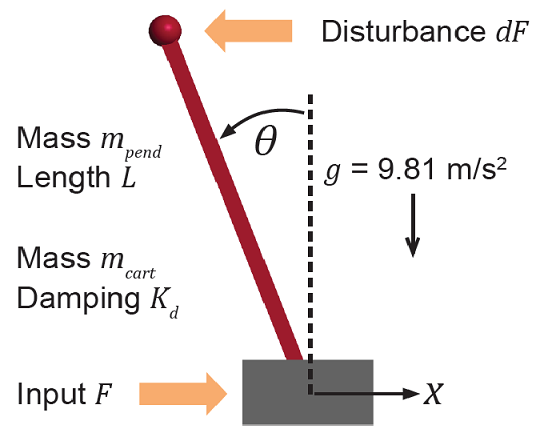
\includegraphics[width=1\linewidth]{Inverted-Pendulum-exemple}
	\caption{Summary of forces applied to an inverted pendulum. The process is similar to figure  \vref{fig:RocketForceSummary}.}
	\label{fig:InvertedPendulum}
\end{figure}


The Cubli is another system known for its instability. It is commonly used in Control Theory to analyze the behavior of a reaction of a wheel inverted system. The advantages of the usage a Cubli is its ability to reach its equilibrium position in microgravity environments, such as asteroids. This is not relevant to the project.

A recent technology facing instability is Segway. A Segway is an application of an Inverted Pendulum to a two wheeled self-balance vehicle. This vehicle requires three body directions instead of the linear motion of an Inverted Pendulum. The study of instability properties of a Segway system would mean the study of elements nonexistent or negligible in a rocket system.

In consideration of the different applications and similarities of the three systems, the Inverted Pendulum will be analyzed to develop a model describing the dynamics of the system, and to design a control system stabilizing the position in vertical position. The objective is to understand and solve the instability properties shared by rocket and inverted pendulum systems.


